\section{Medios de apoyo}

\subsection{Sistema STANLY / ACOS}

\subsection{Sistema LARA}

\subsection{Sistema iADS}

iADS es una herramienta de gestión del espacio aéreo diseñada para mejorar la colaboración en la toma de decisiones entre los organismos civiles y militares en la gestión de la red local. iADS muestra gráficamente la demanda de espacio aéreo y, teniendo en cuenta las limitaciones pertinentes, como los niveles de personal, las configuraciones de los sectores, los valores de los monitores de los sectores y los datos meteorológicos pertinentes, la capacidad del espacio aéreo. iADs proporciona una pantalla visual fácilmente interpretable que permite a los organismos de gestión de la red local comprender plenamente el impacto de las decisiones de asignación del espacio aéreo y proporciona la capacidad de ajustar la asignación del espacio aéreo con el fin de hacer el mejor uso del espacio aéreo disponible.

El conocimiento mutuo de la demanda de espacio aéreo y de los factores que afectan a la demanda, así como una función gráfica "what if" para simular cambios en las reservas solicitadas y en las rutas de las aeronaves, mejora la coordinación y permite optimizar la capacidad del espacio aéreo en beneficio de los usuarios del espacio aéreo civil y militar a nivel local, además de contribuir a la optimización a nivel de red. Este concepto se puede ver en la figura (\ref{fig:iads}).

\begin{figure}[H]
    \centering
    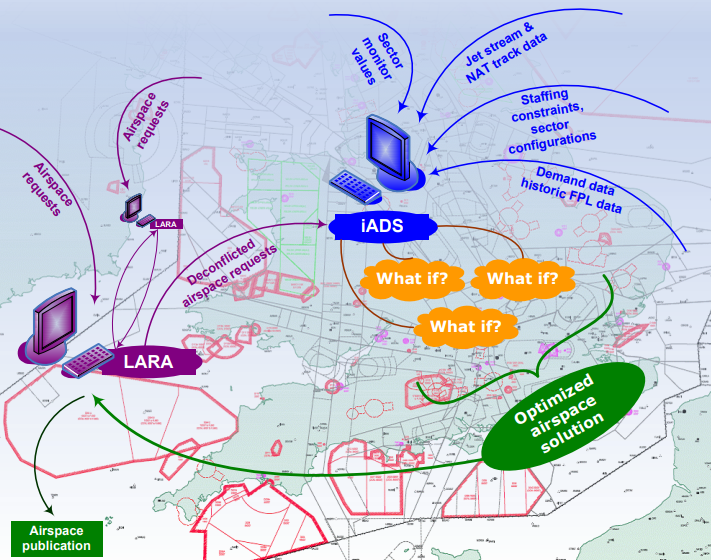
\includegraphics[width=0.7\linewidth]{figuras/iads.png}
    \caption{Concepto iADS.}
    \label{fig:iads}
\end{figure}

iADS se provee mediante un servidor basado en Microsoft (MS) Windows que aloja una base de datos SQL y la aplicación iADS. El servicio está basado en la web y se proporciona a través de una red basada en IP a clientes basados en Windows, utilizando MS Internet Explorer y MS Silverlight. La entrada de datos del sistema en el prototipo se realiza actualmente mediante la transferencia manual de archivos. La entrada de datos manual se realiza mediante la interacción con el cliente. En la figura (\ref{fig:iads_map}) se puede observar la interfaz del programa, donde aparece en el mapa la información relevante.

\begin{figure}[H]
    \centering
    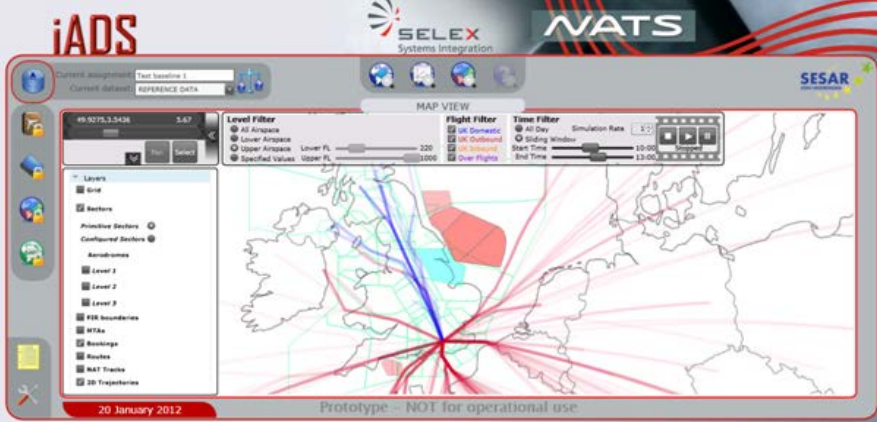
\includegraphics[width=1\linewidth]{figuras/iads_map.png}
    \caption{Vista del mapa en iADS.}
    \label{fig:iads_map}
\end{figure}

El sistema iADS se utiliza para las distintas fases de planificación. La fase 1 de iADS es el inicio de un desarrollo escalonado que apoya los procesos y procedimientos actuales dentro de la toma de decisiones en colaboración con el ASM y el ATFCM. La fase 1 se centra en la toma de decisiones dentro de la escala temporal D-7 a D-3; la fase 2 se centra en la introducción de la toma de decisiones automatizada y controlada por parámetros, y en la optimización del espacio aéreo en el periodo D-3 a D-1; la fase 3 lleva estas mejoras al día de las operaciones. 

El sistema iADS muestra las solicitudes de reserva de espacio aéreo militar, los flujos de tráfico civil y las cargas de los sectores codificadas por colores para poner de manifiesto los desequilibrios de la demanda y la capacidad. iADS permite a los organismos de gestión de la red local plantear escenarios de asignación del espacio aéreo mediante la limitación de niveles o el desplazamiento (tanto geográfico como temporal) de las solicitudes de espacio aéreo, el desvío del tráfico civil y el encasillamiento o la división de los sectores ATC. Esta característica se puede observar en la figura (\ref{fig:iads_request}), donde aparecen las peticiones de espacio aéreo de los distintos usuarios.

\begin{figure}[H]
    \centering
    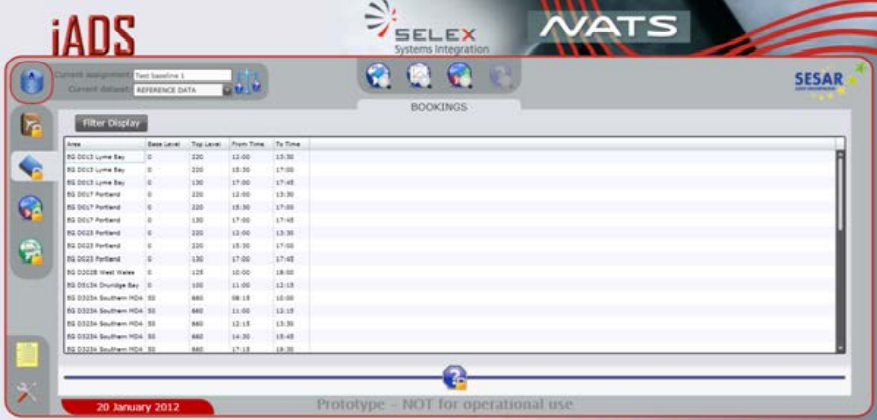
\includegraphics[width=1\linewidth]{figuras/iads_request.png}
    \caption{Peticiones de espacio aéreo en iADS.}
    \label{fig:iads_request}
\end{figure}